% !TEX TS-program = pdflatex
% !TEX encoding = UTF-8 Unicode

% This is a simple template for a LaTeX document using the "article" class.
% See "book", "report", "letter" for other types of document.

\documentclass[12pt]{article} % use larger type; default would be 10pt

\usepackage[utf8]{inputenc} % set input encoding (not needed with XeLaTeX)

\usepackage{kotex}

%%% Examples of Article customizations
% These packages are optional, depending whether you want the features they provide.
% See the LaTeX Companion or other references for full information.

%%% PAGE DIMENSIONS
\usepackage{geometry} % to change the page dimensions
\geometry{a4paper} % or letterpaper (US) or a5paper or....
% \geometry{margin=2in} % for example, change the margins to 2 inches all round
% \geometry{landscape} % set up the page for landscape
%   read geometry.pdf for detailed page layout information

\usepackage{graphicx} % support the \includegraphics command and options

% \usepackage[parfill]{parskip} % Activate to begin paragraphs with an empty line rather than an indent

%%% PACKAGES
\usepackage{booktabs} % for much better looking tables
\usepackage{array} % for better arrays (eg matrices) in maths
\usepackage{paralist} % very flexible & customisable lists (eg. enumerate/itemize, etc.)
\usepackage{verbatim} % adds environment for commenting out blocks of text & for better verbatim
\usepackage{subfig} % make it possible to include more than one captioned figure/table in a single float

\usepackage{makeidx}
\usepackage{titling}
\usepackage{indentfirst}

% These packages are all incorporated in the memoir class to one degree or another...

%%% HEADERS & FOOTERS
\usepackage{fancyhdr} % This should be set AFTER setting up the page geometry
\pagestyle{fancy} % options: empty , plain , fancy
\renewcommand{\headrulewidth}{0pt} % customise the layout...
\lhead{}\chead{}\rhead{}
\lfoot{}\cfoot{\thepage}\rfoot{}

%%% SECTION TITLE APPEARANCE
\usepackage{sectsty}
% \allsectionsfont{\sffamily\mdseries\upshape} % (See the fntguide.pdf for font help)
% (This matches ConTeXt defaults)

%%% ToC (table of contents) APPEARANCE
\usepackage[nottoc,notlof,notlot]{tocbibind} % Put the bibliography in the ToC
\usepackage[titles,subfigure]{tocloft} % Alter the style of the Table of Contents
\renewcommand{\cftsecfont}{\rmfamily\mdseries\upshape}
\renewcommand{\cftsecpagefont}{\rmfamily\mdseries\upshape} % No bold!

%%% ADDITIONAL %%%

\pagenumbering{gobble}
\renewcommand{\thesection}{\Roman{section}} 
\setlength{\parindent}{1cm}
\overfullrule=2cm

%%% BIBLIOGRAPHY %%%




%%% END Article customizations

%%% The "real" document content comes below...

\title{Separation of R- and S- Etodolac Enantiomers by High Performance Liquid Chromatography - Florence Detector after Derivatization with (1R)-(-)-Menthyl Chloroformate}
\author{Hanpil Kang}
\date{} % Activate to display a given date or no date (if empty),
         % otherwise the current date is printed 
\makeindex
\begin{document}

\begin{center}
	\large 졸업논문청구논문
	
	\vskip24mm
	
	\LARGE R- 과 S- Etodolac의 거울상 이성질체의 (1R)-(-)-Menthyl Chloroformate의 유도체화를 통한 HPLC-FLD로 분리
	
	\bigskip
	
	\Large Separation of R- and S- Etodolac Enantiomers by High Performance Liquid Chromatography - Florence Detector after Derivatization with (1R)-(-)-Menthyl Chloroformate
	
	\vfill
	
	강 한 필 ( \textbf{Kang, Hanpil} )
	
	13003
	
	\vskip12mm
	
	과학영재학교 경기과학고등학교
	
	2016
\end{center}
\pagebreak

\begin{center}
	\Large Separation of R- and S- Etodolac Enantiomers by High Performance Liquid Chromatography - Florence Detector after Derivatization with (1R)-(-)-Menthyl Chloroformate
	
	\bigskip
	
	Advisor: Najin, Jeong
	
	by
	
	13003 Kang, Hanpil
	
	\vskip-2mm
	Gyeonggi Science Highschool for the gifted
\end{center}

{
\vskip24mm

\Large
\indent
A thesis submitted to the Gyeonggi Science Highschool in partial fulfillment of the requirements for the graduation. The study was conducted in accordance with Code of Research Ethics\footnote{Declaration of Ethical Conduct in Research: I, as a graduate student of GSHS, hereby declare that I have not committed any acts that may damage the credibility of my research. These include, but are not limited to: falsification, thesis written by someone else, distortion of research findings or plagiarism. I affirm that my thesis contains honest conclusions based on my own careful research under the guidance of my thesis advisor.}.
}

\vfill

{
\Large
\hskip72mm
2015. 6. 19.

\hskip72mm
Approved by

\hskip72mm
Teacher Jeong, Najin (signature)

\hskip72mm
[Thesis Advisor]
}
\pagebreak

\begin{center}
	\LARGE Separation of R- and S- Etodolac Enantiomers by High Performance Liquid Chromatography - Florence Detector after Derivatization with (1R)-(-)-Menthyl Chloroformate
	
	\vskip12mm
	\Large
	강 한 필
	
	\vskip12mm
	
	위 논문은 과학영재학교 경기과학고등학교 졸업논문으로
	
	학위논문심사위원회에서 심사 통과하였음.
\end{center}
\begin{flushright}	
	\Large
	\vskip48mm
	
	2015년 6월 19일
	
	\bigskip
	
	심사위원장 가 나 다(인)
	
	심사위원 메 르 스(인)
	
	심사위원 정 나 진(인)
\end{flushright}
\pagebreak
	




\setcounter{page}{1}
\pagenumbering{roman}

\maketitle

\begin{abstract}
Etodolac, one of nonsteroidal anti-inflammatory drugs(NSAIDs) in R/S- form are shown to be have different pharmacodynamic and pharmacokinetic properties. R- contreats Leukemia, S- treats the symptoms of pain and inflammation. In this research, (1R)-(-)-Menthyl Chloroformate is used to derivate R/S- Etodolac, reacts with Carboxyl group in pyridine catalyst. High Performance Liquid Chromatography - Florence Detector (HPLC-FLD) is used to qualificate two enantiomer of Etodolac, resulting resolution over 1 in standard and serum sample.  
\end{abstract}

\newpage

\begin{center}

	\vskip24mm
	
	\LARGE R- 과 S- Etodolac의 거울상 이성질체의 (1R)-(-)-Menthyl Chloroformate의 유도체화를 통한 HPLC-FLD로 분리
	
	\bigskip

\end{center}

\renewcommand\abstractname{초\hskip6mm 록}
\begin{abstract}
  비스테로이드성 진통제(NSAIDs)의 일종인 에토돌락(Etodolac)의 두 광학 이성질체는 약역학과 약물동태학적으로 다른 성질을 가진다. R-의 형태는 백혈병을 치료에 효과가 있고, S-의 형태는 진통소염 작용을 한다. 이 연구에서는 피리딘 촉매 하에서 (1R)-(-)-멘틸 클로로포메이트를 R/S- 에토돌락의 카르복실기와 반응 시킨다. 고성능 액체 크로마토그래피 – 형광 검출기(HPLC-FLD) 가 두 광학 이성질체를 분리하는데 사용되었으며 해상도 1 이상으로 정성할 수 있다.

\end{abstract}

\newpage

\tableofcontents

\newpage

\listoffigures

\newpage

\listoftables

\newpage



\setcounter{page}{1}
\pagenumbering{arabic}

\section{Introduction}

Etodolac, one of nonsteroidal anti-inflamatory drugs (NSAIDs) is widely used for treating rheumatic and inflammatory diseases. This drug is used as a racemic mixture but the pharmacodynamic and pharmacokinetic properties of two enantimoers are different. R- contreats Leukemia\cite{cite1}, S- treats the symptoms of pain and inflammation. Menthyl Chloroformate was widely used as derivating secondary amine, but also reacts with carboxyl group when catalyst pyridine exists.
High Performance Liquid Chromatography – Florence Detector (HPLC-FLD) and Ultra Performance Liquid Chromatography – Mass spectrometry (UPLC-MS) is powerful machine which can quantify and qualify products. 
In this research, we used HPLC-FLD to detect products made by derivatization of (1R)-(-)-Menthyl Chloroformate to Etodolac. To check two isomers and its structure, UPLC-MS is used.


\begin{figure}[h]
  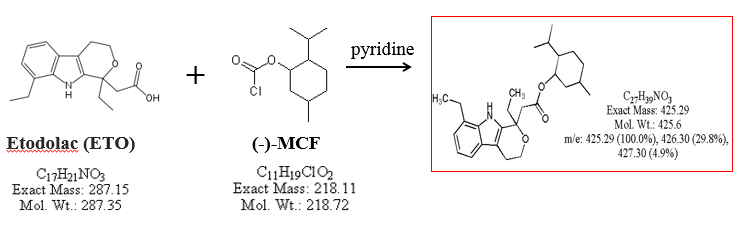
\includegraphics[width=\linewidth]{fig1.png}
  \caption{Etodolac, (-)-MCF and their products.}
  \label{fig:fig1}
\end{figure}

\newpage




\section{Experimental}

\subsection{Chemicals and Reagents}
  R/S-Etodolac was purchased from Tokyo Chemical Industry (Tokyo, Japan).
  (1R)-(-)-Menthyl Chloroformate, Pyridine, L-Proline was purchased from Sigma-Aldrich Chemie (St. Louis, USA).
  Acetonitrile (ACN) and Methanol (MeOH) was purchased from Avantor Performance Materials, Inc (USA).
NaCl was purchased from Merck KGaA (Darmstadt, Germany).

\subsection{High-performance Liquid Chromatography - Florence Detector}
  High-performance liquid chromatography (HPLC) is widely used in analytic chemistry, used to separate, identify or quantify each components in the mixture. Gemini C18 Column was used at flow rate 1.0mL/min, temperature 25'C used with 86.5% MeOH, 13.5% 10mM Acetic Acid.
  Florence Detector is used at wavelength $\lambda$ex= 235 nm; $\lambda$ em= 345 nm.

  Chemstation Software was used for the system control and data processing.


\subsection{Ultra-performance liquid chromatography – Mass Detector}

  Ultra-performance liquid chromatography – Mass Spectrometer (UPLC-MS) is widely used in analytic chemistry, used to separate, identify or quantify each components in the mixture by Mass detection. A mass spectrum is a plot of the ion signal as a function of the mass-to-charge ratio. The spectra are used to determine the elemental or isotopic signature of a sample, the masses of particles and of molecules, and to elucidate the chemical structures of molecules, such as peptides and other chemical compounds
UPLC BEH C18 Column (2.1 x 50mm, 1.7um) was used at flow rate 0.3mL/min, Column temperature was 45'C. Elution conditon follows [Table \ref{tab:table1}]. MassLynx Software was used for the system control and data processing.

\begin{table}[h]
  \begin{center}
    \caption{Elution Condition of UPLC-MS.}
    \label{tab:table1}
    \begin{tabular}{ccc}
      \toprule
      Time(min) & Water(0.1\% Formic Acid) & Methanol (0.1\% Formic Acid) \\
      \midrule
      0 & 20 & 80 \\
      \midrule
      9 & 10 & 90 \\
      \midrule
      11 & 0 & 100 \\
      \midrule
      13 & 0 & 100 \\
      \midrule
      15 & 20 & 80 \\
      \midrule
      17 & 20 & 80 \\
      \bottomrule
    \end{tabular}
  \end{center}
\end{table}

\subsection {Protocol}
  Protocol follows. Add 50uL 50mM etodolac soluted in ACN in 50uL urine. Vortex mixture slightly. Add 900uL of ACN and vortex for 3minute. Centrifuge for 5 minute 13500 round per minute. Take 950uL of upper Layer and evaporate in 40'C in gentle nitrogen stream. Add 160ul 100mM MCF soluted in ACN and 15uL pyridine and 25uL ACN in residue. Sonicate for 10 minute. Add 160uL 100mM proline soluted in distilled water for finalize derivatization. Vortex for 3 minute and place 20 minute at room teperature. Add 28.7mg of NaCl for Liquid-Liquid Extraction and take organic layer and filter.
  Optimization process is done with this protocol.


\subsection {In-vitro test}
 S-etodolac binds well to Albumin than R-etodolac.\cite{cite4} We tried to identify of etodolac enantiomers using stereoselective binding difference of etodolac to albumin.
 Protocol follows.  Add 100uL 50ppm Etodolac. Evaporate in 40'C in gentle nitrogen stream. Add 100uL 50ppm Albumin in pH 7.4 phosphate buffer.
 Albumin purification was done to separate unbound Etodolac. We used Vivaspin 500 to separate protein.
 Protocol follows. In Vivaspin 500 add 100uL diluted water and centrifuge in 10000g for 5 minute. Add 100uL albumin and Etodolac mixture and centrifuge in 10000g for 3 minute. Filter 50uL and add 100 uL buffer and centrifuge in 10000g for 5minute. Repeat 4 times filtering 100uL and adding 100uL buffer and centrifuge in 100g for 5minute. Transfer concentrate and collect filtrate.


\subsection {In-vivo test for rats}
 C57BL/6 mouse (male; 7 w) serum is used for Chrial determination of \linebreak etodolac. Weight of mouse was 20g. Concentration of S-(+)-etodolac is lower than R-(-)-etodolac when injected 20mg/kg from 0 through 70 hour.\cite{cite2}
  Protocol follows. Add 10mg etodolac to 50uL ethanol and vortex for 20s. Add 300uL Tween 80 and vortex for 1 minute and sonicate for 1 minute. After centrifuging 3 seconds, add saline to 10mL. Inject etodolac to mouse.
  200uL was injected to C57 mouse when the weight was 20g.


  

\newpage

\section {Results and Discussion}

\subsection {UPLC-MS Data}


\begin{figure}[h]
  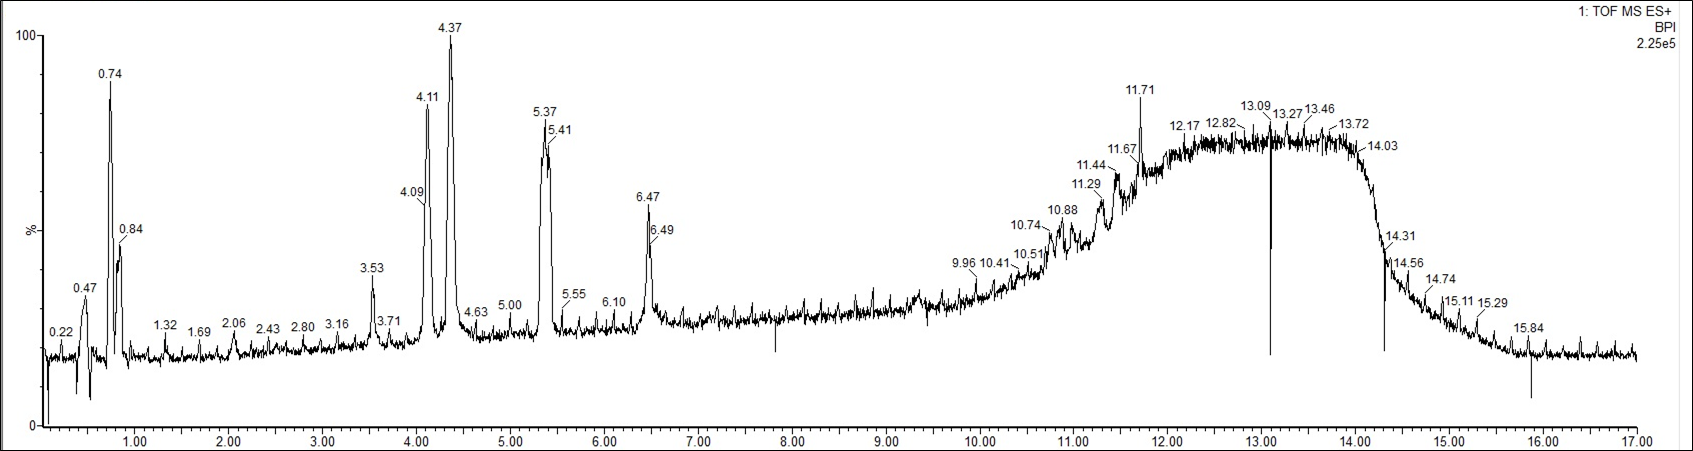
\includegraphics[width=\linewidth]{bpi.png}
  \caption{BPI chromatogram of Menthyl Chloroformate-derivatized Etodolac product }
  \label{fig:fig2}
\end{figure}
\begin{figure}[h]
  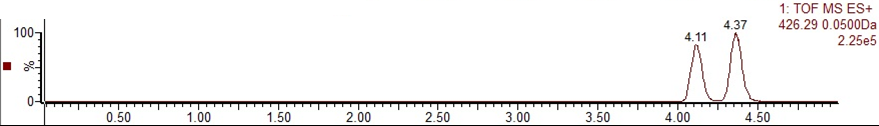
\includegraphics[width=\linewidth]{fig3.png}
  \caption{Extract ion chromatogram of Menthyl Chloroformate-derivatized Etodolac product, [M+H]=426.29}
  \label{fig:fig3}
\end{figure}
\begin{figure}[h!]
  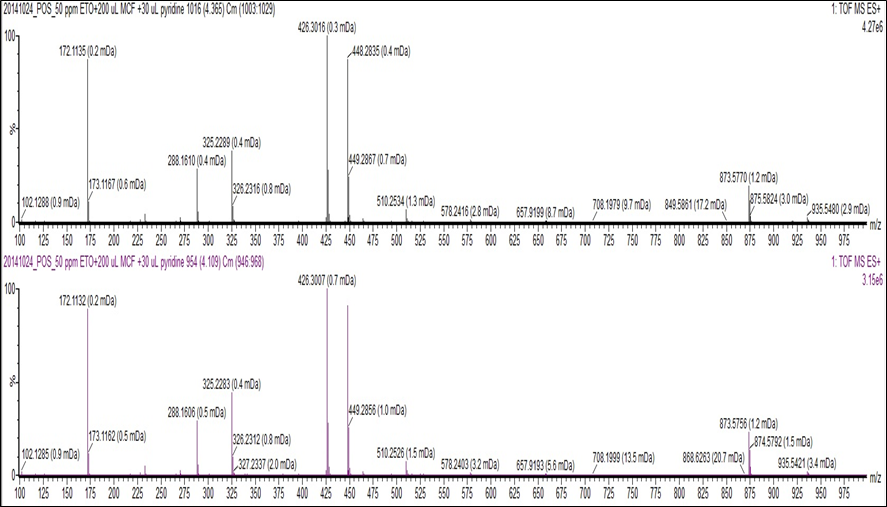
\includegraphics[width=\linewidth]{fig4.png}
  \caption{Mass fragment of peak at retention time 4.11 minute and 4.37 minute.}
  \label{fig:fig4}
\end{figure}

In [Figure \ref{fig:fig4}], mass fragment of peak at 4.11 and 4.37 equals. It means they are not geometric isomer. But they appears at different peak. Mass at 172.1 and 287.15 shows that they have structure of etodolac.\cite{cite3} So we can conclude that they are derivated etodolac. 


\subsection {HPLC-FLD Data}
\begin{figure}[h!]
  \centering
  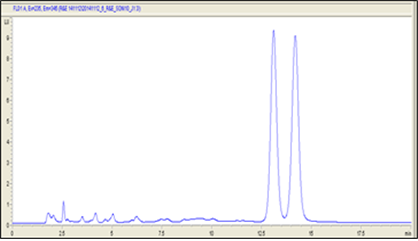
\includegraphics[width=\linewidth]{fig5.png}
  \caption{HPLC-FLD data of protocol}
  \label{fig:fig5}
\end{figure}

In [Figure \ref{fig:fig5}], two peak appears at 13.115, 14.196 minute. Two are enantiomer of etodolac derivatized by Menthyl Chlroforomate. We will call first peak and second peak as peak 1, peak 2. resolution was 1.03.

\subsection{ Protocol Optimization }

  Protocol was optimizated in pyridine volume and sonication time. Peak 2 reacts faster than peak 1. Therefore, we used ratio of peak 1 to verify reaction is almost completed.

\subsubsection {Pyridine Volume}


\begin{figure}[h!]
  \centering
  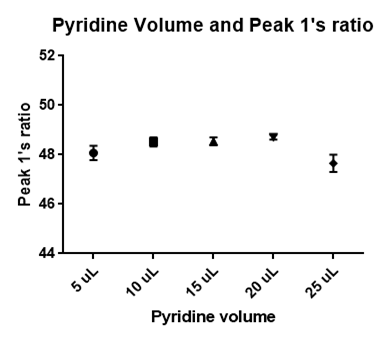
\includegraphics[width=0.6\linewidth]{fig6.png}
  \caption{Pyridine Volume and Peak 1's ratio}
  \label{fig:fig6}
\end{figure}

In [Figure \ref{fig:fig6}],  5uL and 25uL of pyridine volume was significant by t-test. Optimized value was median of not significant pyridine volume, 15uL.

\subsubsection {Sonication time}

\begin{figure}[h!]
  \centering
  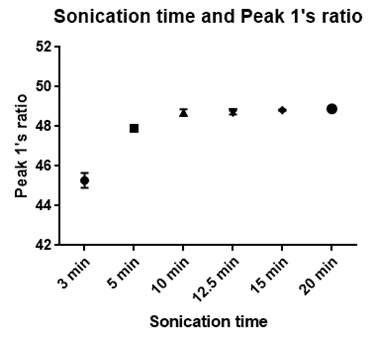
\includegraphics[width=0.6\linewidth]{fig7.png}
  \caption{Sonication time and Peak 1's ratio}
  \label{fig:fig7}
\end{figure}
 In [Figure \ref{fig:fig7}],  3min and 5min was significant by t-test. Optimized value was first not significant time, 10min.



\subsection {In-vitro test}
\begin{figure}[h!]
  \centering
  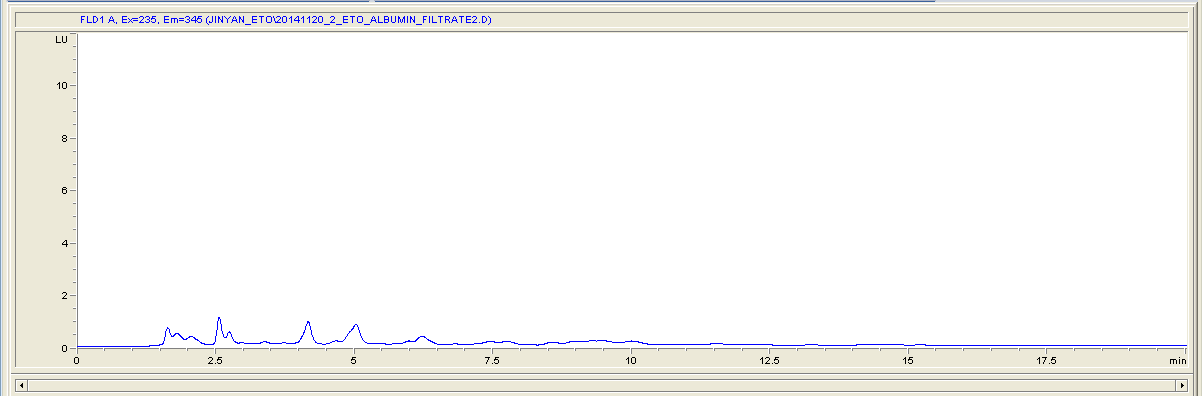
\includegraphics[width=\linewidth]{f9.png}
  \caption{Chromatogram of Filtrate}
  \label{fig:fig9}
\end{figure}
 In vitro test failed. Both Etodolac enantiomers were well binded with protein in short time.


\subsection {In-vivo test for rats}

\begin{figure}[h!]
  \centering
  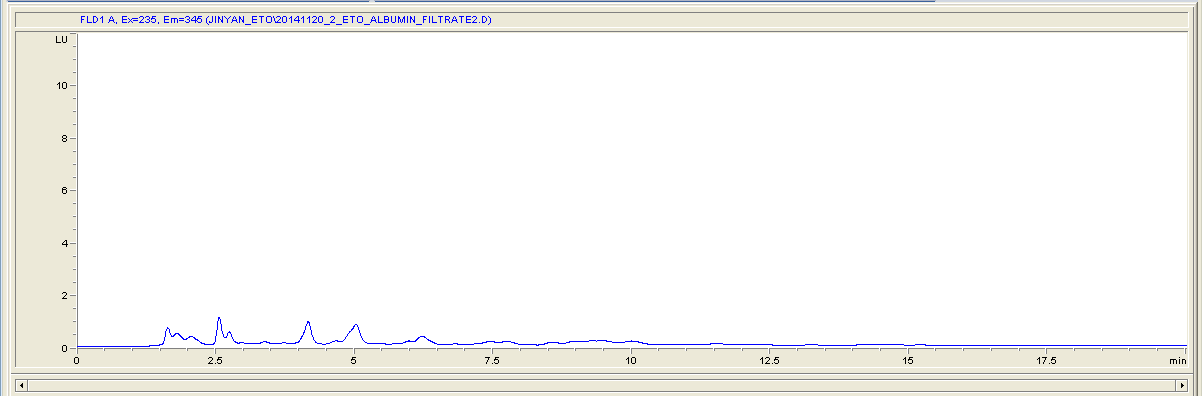
\includegraphics[width=\linewidth]{fig8.png}
  \caption{In vivo test result}
  \label{fig:fig8}
\end{figure}

 In [Figure \ref{fig:fig8}],  1 hour after injection, peak area of Peak 1 is 0.4676 while peak area of Peak 2 is 0.0694. S-etodolac binds faster and Peak 2 has less peak area, which means, Peak 2 is S-etodolac and Peak 1 is R-etodolac.



\newpage

\begin{thebibliography}{100}
\bibitem{cite1}
	Brocks, D. R., Jamali, F., J. Pharm. Sci. 1991, 80, 1058– 1061.


\bibitem{cite2}
        Shi JM et al. / Aeta Pharmacol Sin 2004 Aug; 25 (8): 996-999

\bibitem{cite3}
        Clin Pharmacokinet. Joseph P. Boni, Joan M. Korth-Bradely, Lyette S. Richards, Soong T Chiang, David R. Hicks, Leslie Z. Benet. 2000 Dec, 39(6) 459-469

\bibitem{cite4}
	Chang-Chuan Guo et al. / Journal of Pharmaceutical Analysis  2011;1(3):184-190

\end{thebibliography}

























\end{document}
